\documentclass[10pt, technote]{IEEEtran}
\usepackage[utf8]{inputenc}
\usepackage[english]{babel}
\usepackage[table,xcdraw]{xcolor}
\usepackage[a4paper, footnotesep = 1cm, width=20cm, top=2.5cm, height=25cm, textwidth=18cm, textheight=25cm]{geometry}
%\geometry{showframe}

\usepackage{tikz}
\usepackage{amsmath}
\usepackage{amsfonts}
\usepackage{amssymb}
\usepackage{float}
\usepackage{graphicx}
\usepackage{caption}
\usepackage{subcaption}
\usepackage{multicol}
\usepackage{multirow}
\setlength{\doublerulesep}{\arrayrulewidth}
\usepackage{booktabs}
\usepackage{cite}

\usepackage{hyperref}
\hypersetup{
    colorlinks=true,
    linkcolor=blue,
    filecolor=magenta,      
    urlcolor=blue,
    citecolor=blue,    
}

\newcommand{\quotes}[1]{``#1''}
\usepackage{array}
\newcolumntype{C}[1]{>{\centering\let\newline\\\arraybackslash\hspace{0pt}}m{#1}}
\usepackage[american]{circuitikz}
\usetikzlibrary{calc}
\usepackage{fancyhdr}
\usepackage{units} 

\graphicspath{./Imagenes}

\pagestyle{fancy}
\fancyhf{}
\lhead{22.05 - ASSD}
\rhead{Mechoulam, Lambertucci, Rodriguez, Londero Bonaparte}
\rfoot{Página \thepage}

\usepackage[procnames]{listings}
\begin{document}

%%%%%%%%%%%%%%%%%%%%%%%%%
%		Caratula		%
%%%%%%%%%%%%%%%%%%%%%%%%%

\begin{titlepage}
\newcommand{\HRule}{\rule{\linewidth}{0.5mm}}
\center
\mbox{\textsc{\LARGE \bfseries {Instituto Tecnológico de Buenos Aires}}}\\[1.5cm]
\textsc{\Large 22.05 Análisis de Señales y Sistemas Digitales}\\[0.5cm]


\HRule \\[0.6cm]
{ \Huge \bfseries Trabajo práctico N$^{\circ}$4}\\[0.4cm]
{ \Large \bfseries Entrega N$^{\circ}$2}\\[0.4cm] 
\HRule \\[1.5cm]


{\large

\emph{Grupo 3}\\
\vspace{3px}

\begin{tabular}{lr} 	
\textsc{Mechoulam}, Alan  &  58438\\
\textsc{Lambertucci}, Guido Enrique  & 58009 \\
\textsc{Rodriguez Turco}, Martín Sebastian  & 56629 \\
\textsc{Londero Bonaparte}, Tomás Guillermo  & 58150 \\
\end{tabular}

\vspace{20px}

\emph{Profesores}\\
Jacoby, Daniel Andres\\
Belaustegui Goitia, Carlos F.\\
Iribarren, Rodrigo Iñaki\\
\vspace{3px}
%\textsc{} \\	

\vspace{100px}

\begin{tabular}{ll}

Presentado: & ??/07/20\\

\end{tabular}

}

\vfill

\end{titlepage}


%%%%%%%%%%%%%%%%%%%%%
%		Indice		%
%%%%%%%%%%%%%%%%%%%%%

%\tableofcontents
%\newpage

%%%%%%%%%%%%%%%%%%%%%
%		Informe		%
%%%%%%%%%%%%%%%%%%%%%

\textbf{\textit{En el siguiente trabajo se presenta la investigación y desarrollo de un proceso de seguimiento de un objeto en tiempo real siendo conocida su posición inicial. Se utilizaron los algoritmos de Shi-Tomasi, Optical Flow de Lucas-Kanade, filtros de Kalman, de probabilidad de distribución de color y de correlación para lograr robustez ante cambios en la iluminación, oclusiones parciales o totales y cambios bruscos en la trayectoria incluso durante una oclusión.}}

\section{Introducción}
Una imagen puede ser interpretada como una función bidimensional $f\left( x, y\right)$, donde tanto $x$ como $y$ representan en un plano el espacio visualizado, mientras que la misma función $f\left( x, y\right)$ es la intensidad de la imagen bajo un punto dado. Cuando $x$, $y$ y $f\left( x, y\right)$ son valores cuantizados y discretizados, la imagen se transforma en una imagen digital.

%f(x, y) como un campo vectorial cuya salida es un vector de intensidad y frecuencia
	 	
El procesamiento de dichas se define como el conjunto de técnicas aplicadas a estas imágenes, con el objetivo extraer información de ellas. Estas actividades cubren un campo que abarca un sin fin de aplicaciones, ya que se vale de maquinas capaces de detectar la totalidad del espectro electromagnético. Esto significa que se pueden obtener imágenes generadas por fuentes que captan información la cual para los humanos no se asocian con imágenes propiamente dichas, como lo son las ondas de radio, entre tantas otras.
	
Es posible considerar tres tipos de procesos computarizados en el procesamiento de imágenes, basándose en el nivel de tratamiento que se aplique, siendo así clasificados en bajo, medio y alto nivel. Los primeros incluyen actividades tales como reducción de ruido y aumento de contraste, tareas caracterizadas por el hecho de que tanto la entrada como la salida son imágenes. Las actividades de medio nivel de procesamiento incluyen trabajos de segmentación, es decir, identificar regiones u objetos dentro de las imágenes, descripción y clasificación de dichos elementos. Es así que esta categoría es destacada por sus salidas, ya que suelen ser información extraída de las imágenes a la entrada. Por último, los procesos de alto nivel se caracterizan por no solo reconocer objetos y analizarlos, sino también por darles un tratado normalmente asociado con la visión, tales así como ``darles sentido'' \cite{ref:intro1}.
	
Dada una señal continua a la entrada del sistema, una imagen sufre de dos procesos claves: \textbf{cuantización} y \textbf{discretización}. Si bien ambos refieren a tomar variables continuas y almacenarlas en memoria como variables discretas, se realiza esta diferenciación entre ambas ya que la primera hace referencia a la amplitud de la señal mientras que la segunda a coordenadas, que para el caso del estudio de imágenes, se refiere a pixeles. Estos son el mínimo elemento que compone una imagen digital y se pueden pensar como un cuadrado de color uniforme.
	
Ejemplificando lo anterior, se toma una entrada al sistema, como puede ser la presentada en la Figura (\ref{fig:disc1}), la cual, como ya se ha mencionado, es continua en $x$, $y$ y $f(x,y)$.
\begin{figure}[H]
\centering
	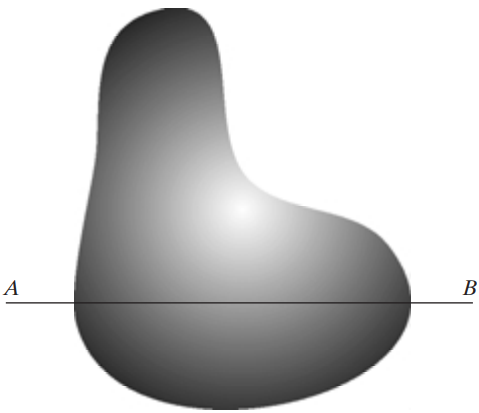
\includegraphics[width=0.3\textwidth]{Imagenes/Digitalizacion_1.png}
	\caption{Entrada continua al sistema.}
	\label{fig:disc1}
\end{figure}

Por lo tanto, se deben tomar coordenadas finitas, por ejemplo, aquellas que se encuentran sobre la recta AB, y asignarle a cada una un valor dado de amplitud. En la Figura~(\ref{fig:disc2}) se observa como una recta continua paralela al eje $x$ (horizontal), la cual posee ciertas variaciones aleatorias dadas por el ruido existente, es dividida en una cierta cantidad de posiciones equiespaciadas (discretización), marcadas con cuadrados blancos sobre la curva, asignándoles un nivel específico en la escala de grises (cuantización), marcado con una linea negra por la izquierda de dicha escala.
\begin{figure}[H]
\centering
	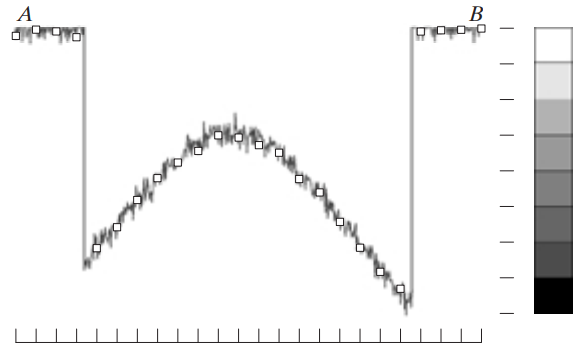
\includegraphics[width=0.4\textwidth]{Imagenes/Digitalizacion_2.png}
	\caption{Amplitud de la escala de grises en la recta AB y muestreo de valores.}
	\label{fig:disc2}
\end{figure}

Realizando el mismo proceso para todos los niveles de discretización en el eje $y$ (vertical), se obtiene finalmente una imagen digitalizada, la cual se la compara a continuación con la original \cite{ref:digit1}.
\begin{figure}[H]
\centering
	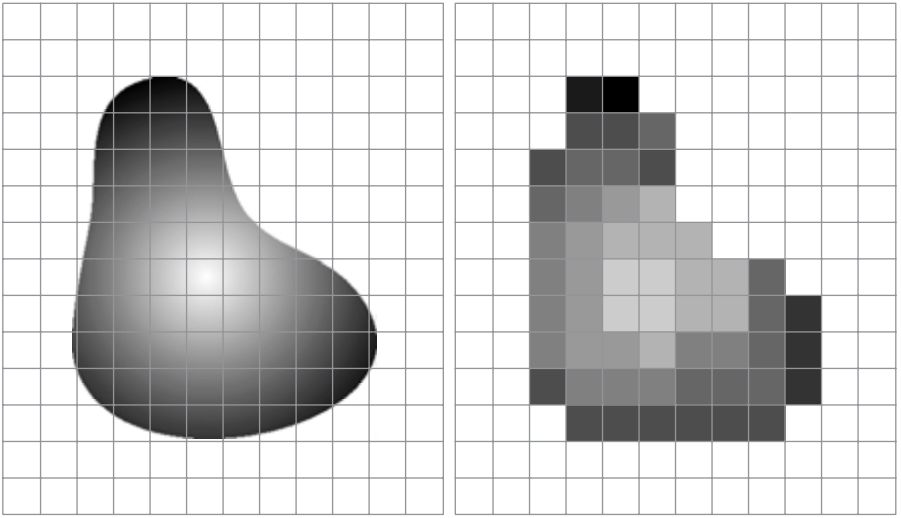
\includegraphics[width=0.5\textwidth]{Imagenes/Digitalizacion_3.png}
	\caption{Imagen original comparada con la imagen digitalizada a procesar.}
	\label{fig:disc3}
\end{figure}

Este trabajo se centra en procesos de medio nivel. Dicha definición es muy amplia, por lo cual es necesario acotar este camino. Es por ello que se decidió focalizarse en el seguimiento de objetos en imágenes en movimiento. Se buscó que, dada ciertas condiciones iniciales conocidas (brindadas por el usuario) en una imagen en movimiento en tiempo real, tomar un conjunto de datos de $x$, $y$ y $f(x,y)$ para así seleccionar un elemento y seguir su trayectoria a través del tiempo. Como hipótesis se plantea que:
\begin{itemize}
\item El objeto no cambiará rápidamente de color ni su iluminación o exposición-
\end{itemize}
Para esto, se utilizaron los algoritmos de Shi-Tomasi, Optical Flow de Lucas-Kanade asimismo como filtros de correlación, de Kalman y de probabilidad de distribución de color.
	
\section{Investigación}
\subsection{Optical Flow} 
El campo de movimiento de una imagen es el movimiento real del objeto en el espacio proyectado sobre el plano de la imagen. El Optical Flow (flujo óptico) se define como el flujo de la intensidad en escala de grises en el plano de la imagen, a medida que evoluciona en el tiempo. También se puede interpretar el flujo de la imagen como el movimiento aparente de esta basado en la percepción visual, teniendo dimensión de velocidad $\vec{V}= (V_x \ , \ V_y)$. Si el Optical Flow se determina de dos imágenes consecutivas, aparece un vector de desplazamiento $\vec{d}$ de las cualidades elegidas, entre el cuadro n y el n+1.
\begin{figure}[H]
		\centering
		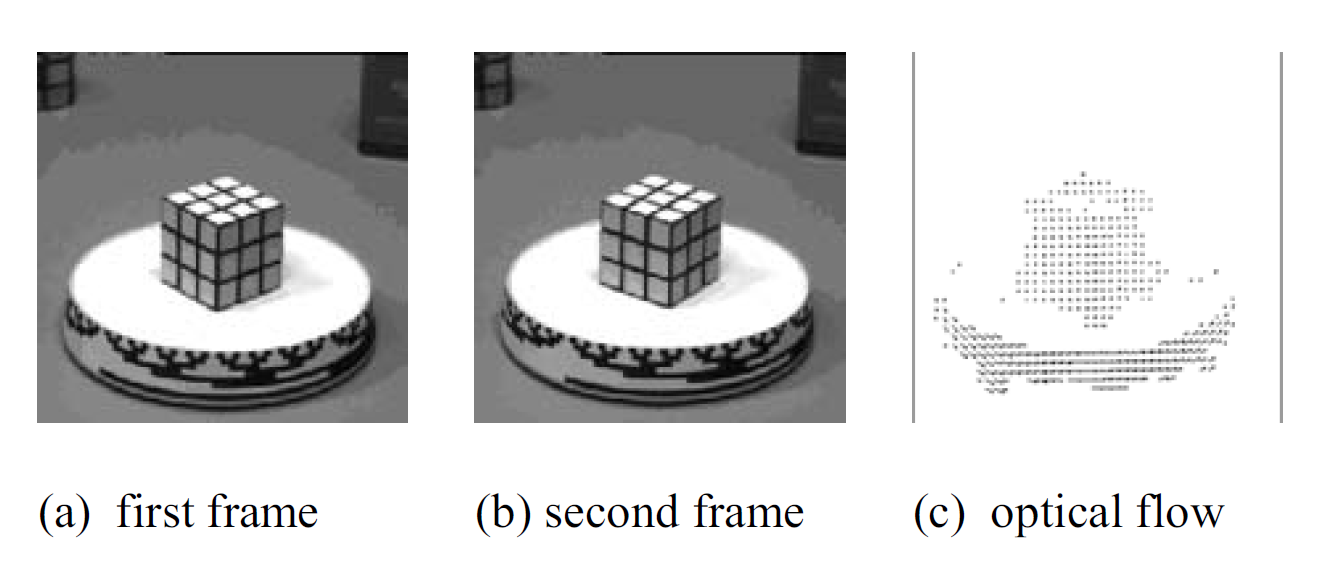
\includegraphics[width=0.5\textwidth]{Imagenes/opticalflowrubick.png}
		\caption{Cubo de rubik rotando en una mesa.}
		\label{fig:opticalflow1}
\end{figure}
Para la implementación del algoritmo existen varios caminos, como lo es, por ejemplo, el basado en calculo de gradientes de la imagen total. Existe otro que utiliza solo ciertos puntos que se determinan constantes de la imagen. El el presente se emplea el método piramidal de Lucas-Kanade.

\subsubsection{Lucas-Kanade} 
Este algoritmo consta del uso de información obtenida a partir de la intensidad del gradiente espacial para buscar la posición que mejor se acomoda a una imagen en movimiento \cite{ref:lucas-kanade} \cite{ref:lucas-kanade2}. Algunas de las hipótesis que postula Lucas-Kanade son:
\begin{itemize}
\item Los movimientos entre cuadros consecutivos son pequeños. Tan pequeños como un pixel.
\item La intensidad de los objeto se mantiene constante cuadro a cuadro.
\end{itemize} 
Este algoritmo se basa en el principio de ``divide y conquistarás'' al realizar la tarea de detectar movimiento en toda la imagen en problemas más sencillos. El proceso consta de dividir la pantalla en un árbol cuaternario. Esto lo hace debido a que se requiere que las hipótesis de Lucas-Kanade deben cumplirse, se toma una pequeña parte de la imagen, del menor tamaño posible, donde tienden a cumplirse las condiciones necesarias del algoritmo. De allí se calcula recursivamente cada partición hasta el primer nivel.
\begin{figure}[H]
		\centering
		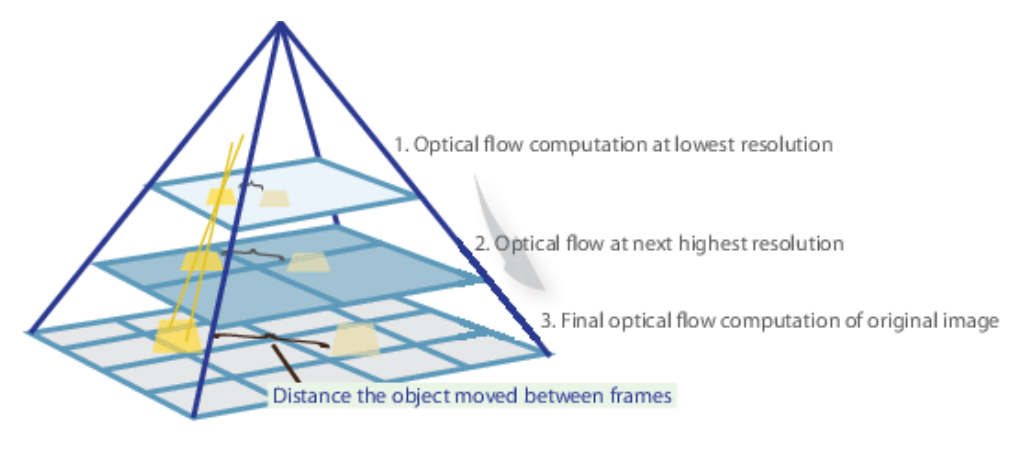
\includegraphics[width=0.5\textwidth]{Imagenes/op.png}
		\caption{Cálculo del Optical Flow.}
		\label{fig:opticalflow1}
\end{figure}
\subsection{Shi-Tomasi}

Por su parte, el algoritmo de Shi-Tomasi se basa en el algoritmo de Harris para la detección de bordes. El funcionamiento del algoritmo se basa en asignarle un valor a cada pixel del bitmap recibido, y si el valor del pixel es mayor a cierto límite se determina que este corresponde a una esquina. El valor asignado al pixel se obtiene utilizando dos autovalores de una matriz Z. Una función recibe estos autovalores, para poder manipularlos y devolver el valor.
La diferenciación entre el algoritmo de Harris y el de Shi-Tomasi, es que mientras Harris utiliza la función mencionada previamente, Shi-Tomasi decide utilizar únicamente los autovalores \cite{ref:shi-tomasi}.
\\ Los valores de cada pixel se determinan de la siguiente manera:

\begin{figure}[H]
\begin{align}
R= det(Z) - k (trace Z )^2 \\
det(Z)= \lambda_1 \cdot \lambda_2 \\
trace Z = \lambda_1 + \lambda_2
\end{align}
\label{eq:harris}
\caption{Valor de pixel para algoritmo de Harris}
\end{figure}

\begin{figure}[H]
\begin{align}
R= min(\lambda_1 , \lambda_2)
\end{align}
\label{eq:shitom}
\caption{Valor de pixel para algoritmo de Shi-Tomasi}
\end{figure}

\begin{figure}[H]
\centering
	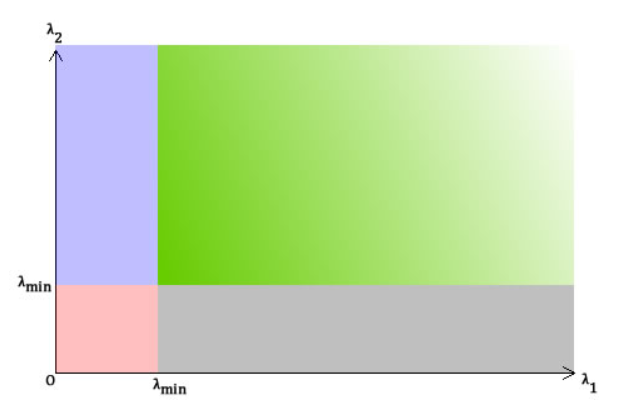
\includegraphics[width=0.4\textwidth]{Imagenes/shitom.png}
	\caption{Detección de bordes Shi-Tomasi.}
	\label{fig:shitom}

\end{figure}
\begin{itemize}
\item La zona verde corresponde a ambos $\lambda_1 \ y \ \lambda_2 $ mayores al valor límite, por lo que estos píxeles son tomados como esquina.
\item La zona azul y gris corresponden a que uno de los autovalores es menor al límite.
\item La zona roja corresponden a ambos autovalores menores al mínimo.
\end{itemize}
\subsection{Filtro de Kalman}
El filtro de Kalman es un filtro recursivo que busca estimar el estado de un sistema dinámico lineal discretizado de dimensión $n$ mediante una serie mediciones con ruido a partir de la descripción del modelo físico que rige las variables del vector de estado\cite{ref:kalman1}, \cite{ref:kalman2}.

\subsubsection{Planteo del problema}
Dado un proceso estocástico lineal en tiempo discreto definido por

\begin{equation}
x_k = Ax_{k-1} + w_{k-1} \footnote{Se omitió por simplicidad la función de control.}
\end{equation}

donde $x_k \in \mathcal{R}^{N}$ y siendo una medición en tiempo $k$ definida por

\begin{equation}
z_k = Hx_k + v_k
\end{equation}

con $z_k \in \mathcal{R}^m$, donde $w_k$ y $v_k$ son variables aleatorias que representan el ruido del proceso y de observación respectivamente, las cuales se asumen que son independientes entre sí y con distribuciones de probabilidad normales multivariadas definidas como

\[ p(w) \sim N(0, Q) \]

\[ p(v) \sim N(0, R) \]

donde $Q$ y $R$ son las matrices de covarianza del ruido del proceso y ruido de medición respectivamente, las cuales se asumen constantes; donde la matriz de transición de estados $A$ de dimensión $n\times n$ \textemdash siendo $n$ la dimensión de estados dinámicos del modelo\textemdash \ define la relación entre estados del paso $k-1$ al paso $k$ sin contar el ruido del proceso; donde la matriz de transición de observación $H$ de dimensión $m\times n$ \textemdash siendo $m$ la dimensión del vector de medición\textemdash \  fija la relación entre el espacio de  los observables medidos y el espacio de las variables del vector de estados, sin contar el ruido de medición; y finalmente donde el estado del filtro puede representarse como $\hat{x}_{k|k}$ y $P_{k|k}$, siendo estos el estimador del vector de estados a posteriori dadas las mediciones hasta un tiempo $k$, y el estimador de la matriz de covariaza a posteriori dadas las mediciones hasta un tiempo $k$ respectivamente. Se puede definir la operación del filtro de Kalman separando a esta en dos fases: la predicción, y la corrección.

\subsubsection{Ecuaciones de predicción}

\begin{equation}
\hat{x}_{k|k-1} = A\hat{x}_{k-1|k-1}
\end{equation}
\begin{equation}
P_{k|k-1} = AP_{k-1|k-1}A^T + Q
\end{equation}

\subsubsection{Ecuaciones de observación}

\begin{equation}
\hat{x}_{k|k} = \hat{x}_{k|k-1} + K_k y_k
\end{equation}
\begin{equation}
P_{k|k} = (\mathbb{I}-K_kH)P_{k|k-1}
\end{equation}

donde,

\begin{equation}
y_k = z_k - H\hat{x}_{k|k-1}
\end{equation}
\begin{equation}
S_k = HP_{k|k-1}H^T + R_k
\end{equation}
\begin{equation}
K_k = P_{k|k-1}H^TS_k^{-1}
\end{equation}

\begin{figure}[H]
		\centering
		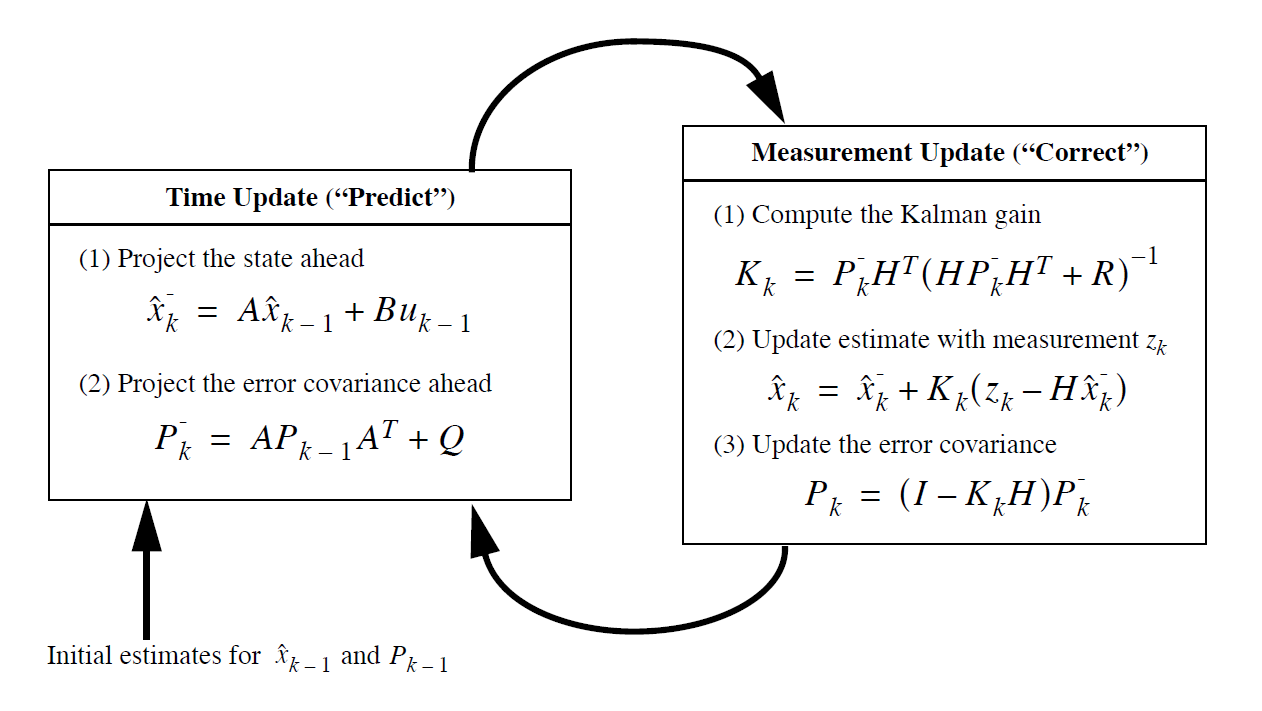
\includegraphics[width=0.5\textwidth]{Imagenes/kalman1.png}
		\caption{Funcionamiento completo del filtro Kalman simple \cite{ref:kalman2}.}
		\label{fig:kalman1}
\end{figure}




 En la Figura (\ref{fig:kalman-comp}) se puede observar el funcionamiento del algoritmo con un vector de estados dinámicos de dimensión dos compuesto por las coordenadas $(x,y)$ sobre el plano cartesiano. Realizando mediciones periódicamente, se comparan dos curvas. Por un lado, una senoidal con un ruido gaussiano montado sobre ella, simulando una serie de mediciones con ruido, y por el otro lado, la estimación obtenida a partir del filtro desarrollado.

\begin{figure}[H]
\centering
	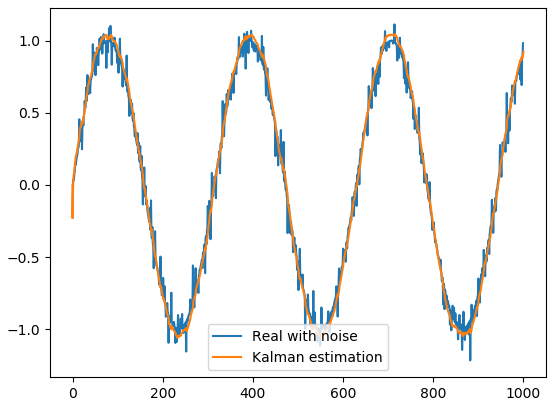
\includegraphics[width=0.4\textwidth]{Imagenes/Kalman_test_1.png}
	\caption{Seno con ruido comparada con estimación de Kalman.}
	\label{fig:kalman-comp}
\end{figure}

\subsection{Filtros de Correlación:}
\label{sec:corr}
El filtro de correlación o también conocido como ``Matched Filter'' \cite{ref:Corr} en inglés, se obtiene al calcular la correlación de una señal conocida, o ``kernel'', con una señal desconocida con el propósito de detectar este kernel en la última señal. Esto último es equivalente a convolucionar la señal desconocida con la inversión temporal del conjugado de la conocida. Este filtro es el óptimo lineal que maximiza la relación señal a ruido (SNR) en presencia de ruido aditivo.

Existen diversas maneras de calcular esta correlación, los dos métodos propuestos fueron:
\begin{itemize}
\item Cuadrados mínimos:
Se basa en el cálculo de cuadrados mínimos entre el kernel y la imagen mientras se realiza la convolución y corresponde a la siguiente ecuación
\begin{align}
R(x,y) = \frac{\Sigma_{x',y'} \left( T(x',y') - I(x+x',y+y') \right)^2}{\sqrt{\Sigma_{x',y'} T(x',y')^2  \cdot \Sigma_{x',y'}  I(x+x',y+y')^2}}
\end{align}
\item Estimación de la correlación:
Se calcula la correlación por definición del frame con respecto al kernel a medida que se desliza por la imagen, le corresponde la siguiente fórmula
\begin{align}
R(x,y) = \frac{\Sigma_{x',y'} \left( T(x',y') \cdot I(x+x',y+y') \right)}{\sqrt{\Sigma_{x',y'} T(x',y')^2  \cdot \Sigma_{x',y'}  I(x+x',y+y')^2}}
\end{align}
\end{itemize}
Donde R es la función de resultado, I la señal desconocida, y T el template o kernel.

En la Figura (\ref{fig:corrtest}) se puede observar una imagen y el resultado del cálculo de correlación utilizando la correlación por cuadrados mínimos y por correlación.

\begin{figure}[H]
\centering
	\begin{subfigure}{.4\textwidth}
		\centering
		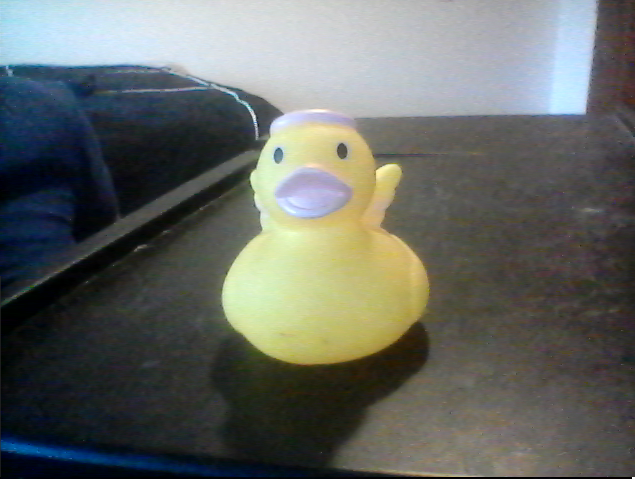
\includegraphics[width=0.8\textwidth]{Imagenes/Original.png}
		\caption{Imagen Fuente.}
		\label{fig:original}
	\end{subfigure}
	\begin{subfigure}{.4\textwidth}
		\centering
		
\includegraphics[width=0.8\textwidth]{Imagenes/Correlation.png}
		\caption{Correlación utilizando definición.}
		\label{fig:corr}
	\end{subfigure}
		\begin{subfigure}{.4\textwidth}
		\centering
		
\includegraphics[width=0.8\textwidth]{Imagenes/SQDIFF.png}
		\caption{Correlación utilizando cuadrados mínimos.}
		\label{fig:sqdiff}
	\end{subfigure}
	\begin{subfigure}{.1\textwidth}
		\centering
		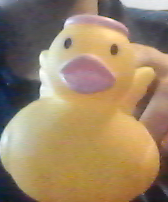
\includegraphics[width=1.2\textwidth]{Imagenes/kernel.png}
		\caption{Kernel.}
		\label{fig:kernel}
	\end{subfigure}
	\caption{Aplicación del algoritmo de correlación.}
	\label{fig:corrtest}
\end{figure}
Se puede apreciar como el punto más oscuro de la pantalla indica el punto de mayor correlación entre la imagen fuente y el kernel seleccionado para el algoritmo de cuadrados mínimos (Figura (\ref{fig:sqdiff})) mientras que el mas claro indica la mayor correlación para el otro (Figura (\ref{fig:corr})). 

\subsection{Filtros basados en distribución de probabilidad de Hue:}
Los filtros de color tradicionales usualmente se basan en la detección de un color especifico con la adición de una cierta tolerancia para poder incluir una gama de colores más amplia. Sin embargo dicha elección resulta ser demasiado restrictiva cuando aparecen sombras o cambios de iluminación. Es por eso que una alternativa más permisiva es la de utilizar mascaras que permitan el paso de ciertos colores según una función de masa de probabilidad dada. Dicha distribución se computa usando como semilla el objeto que deseamos seguir.
\begin{figure}[H]
\centering
	\begin{subfigure}{.1\textwidth}
		\centering
		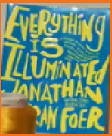
\includegraphics[width=1.2\textwidth]{Imagenes/camshift_kernel.png}
		\caption{Kernel}
		\label{fig:kernelHistFilter}
	\end{subfigure}
\end{figure}

\subsection{Espacios de Color HSV y CIE-L*a*b*:}
El espacio de color HSV, o hue-saturation-value logra representar a un color mediante tres ejes distintos. A diferencia del espacio de colores usual, RGB, que describe un color mediante sus componentes de rojo, verde y azul, en el espacio HSV se describe mediante la oscuridad/luminosidad del color, al cual se le asigna la componente value; la cantidad de pigmentación o pureza del color, al cual se le asigna la componente de saturación; y finalmente la componente de hue, que describe el \textit{chroma} según la teoría de colores, es decir la posición en la rueda de colores.

\begin{figure}[H]
		\centering
		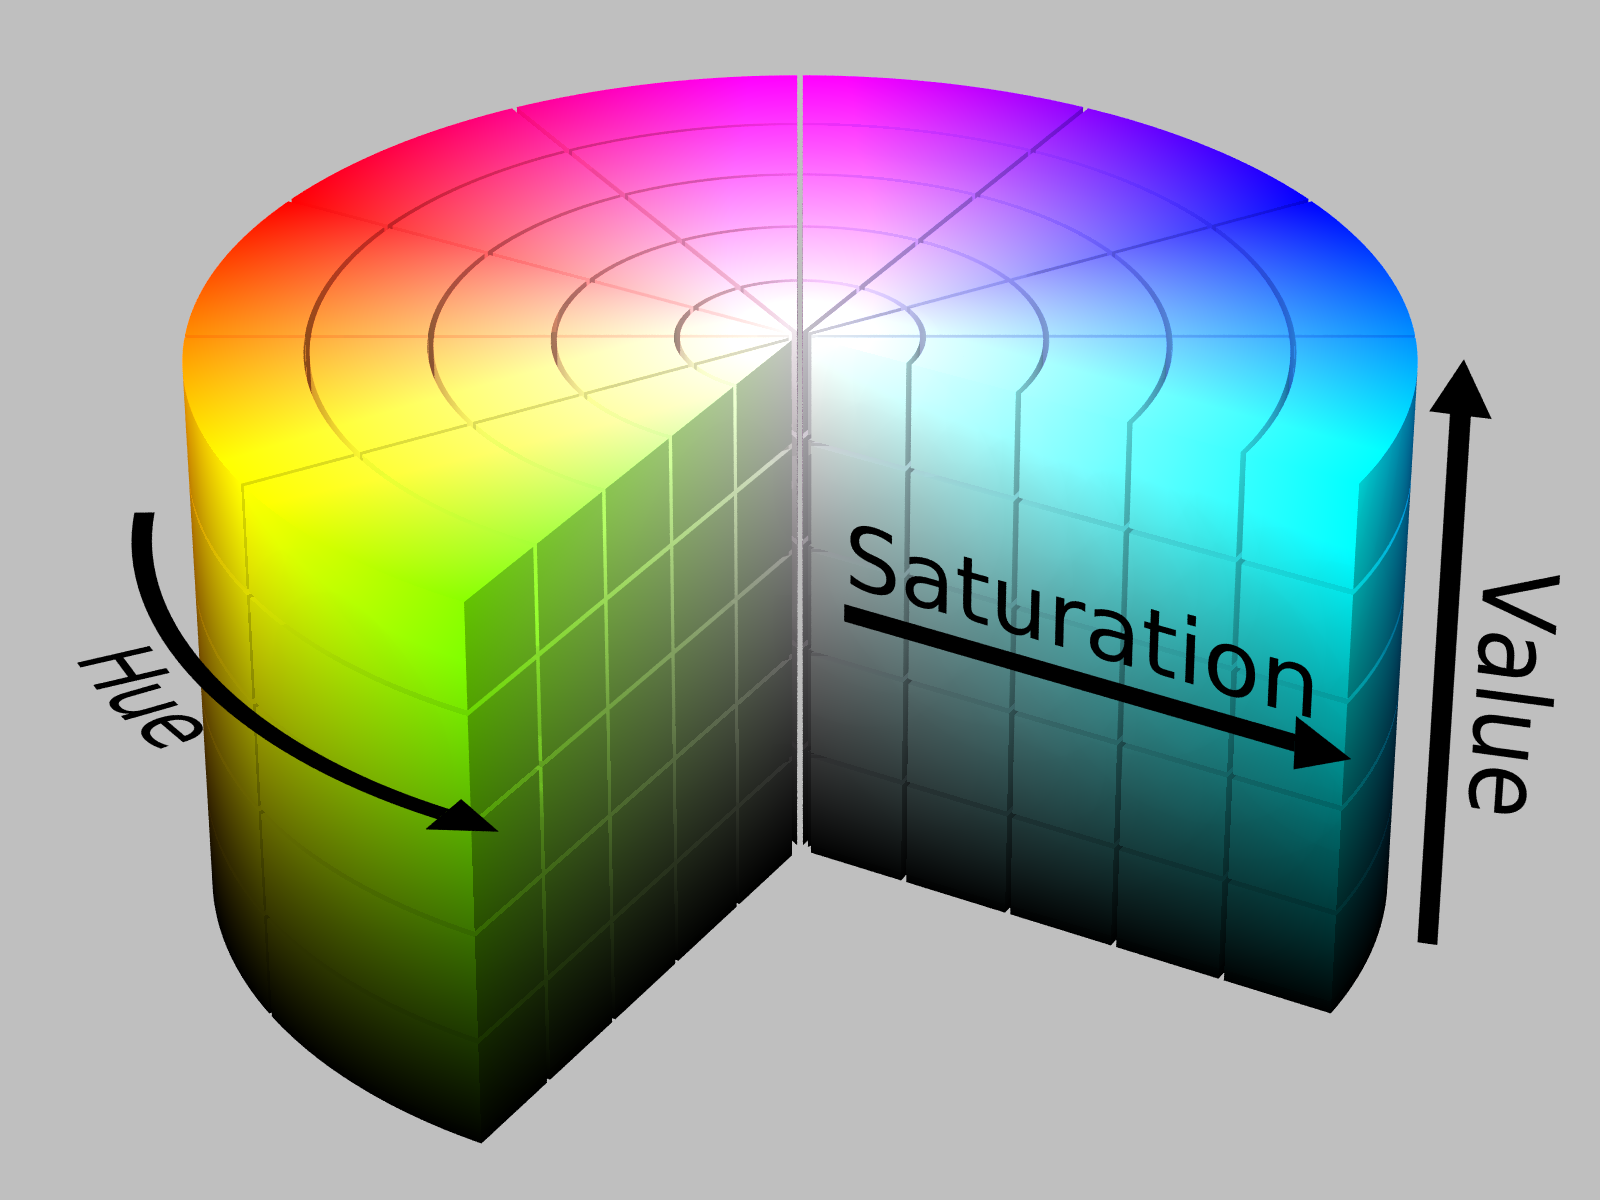
\includegraphics[width=0.3\textwidth]{Imagenes/hsv.png}
		\caption{Espacio de colores HSV representado como un cilindro.}
		\label{fig:hsv}
\end{figure}

Este espacio se puede representar como un cilindro, como se demuestra en la Figura (\ref{fig:hsv}). Si bien la componente de value representa la oscuridad/luminosidad de un color, este modelo es incorrecto debido a que presenta uniformidades. Es por esto, que para obtener una verdadera representación de luminosidad se utiliza el espacio Lab.
El espacio de color L*a*b* de la comisión internacional en iluminación o CIE por sus siglas en francés es un espacio de color perceptualmente uniforme que representa a un color mediante tres parámetros: lightness, a y b, siendo lightness un modelo correctamente calculado e uniforme de la luminosidad de un color, y a y b las componentes de rojo/verde y amarillo/azul del color respectivamente\footnote{Imagen atribuida en \href{https://opentextbc.ca/graphicdesign/chapter/colour-science/}{https:\slash \slash opentextbc.ca\slash graphicdesign\slash chapter\slash colour-science\slash}}.
\begin{figure}[H]
		\centering
		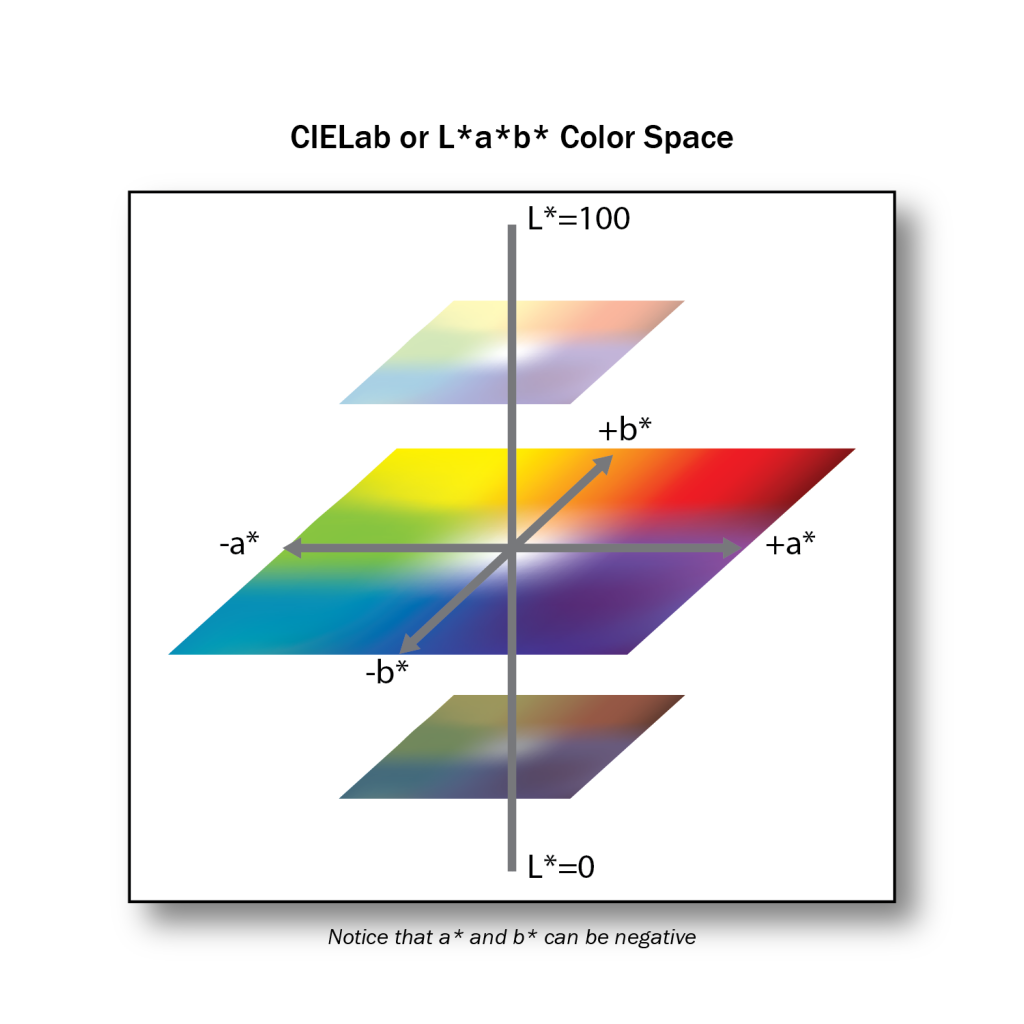
\includegraphics[width=0.3\textwidth]{Imagenes/lab.png}
		\caption{Espacio de colores CIE-Lab en coordenadas cartesianas.}
		\label{fig:lab}
\end{figure}



\section{Aportes y Desarrollo}
\subsection{Implementación}


\section{Trabajo en futuro}
Algunas mejoras que pueden ser implementadas en futuros desarrollos son:
\begin{itemize}
\item Trackeado multiobjeto: \\
Da la opción al usuario de trackear mas de un objeto en la pantalla, utilizando filtros de color diferenciados por cada objeto.
\item Filtro de Kalman donde la matriz de covarianza de medición no sea constante: \\
En el modelo utilizado actualmente la matriz de covarianza es constante, esto asume que la presición de  medición es fija. Esto último no suele ser verdad en la realidad. Una mejora es la introducción de modificaciones en la matriz de covarianza de manera dinámica así el filtro proporcionaría mejores predicciones. 


\item Filtros de correlación:\\
El uso de filtros de correlación tomando como cuadro inicial la selección del usuario se calcula  la correlación con toda la pantalla entre cuadros, donde la correlación sea mayor será mas probable la coincidencia.

\item Invarianza ante cambios de iluminación:\\
El cambio de iluminación impacta directamente sobre el color percibido. Esto afecta directamente a nuestra técnica de filtrado por color. Es por eso que se desean explorar formas de hacer más robusto al sistema ante estos cambios.

\item Filtro de sensibilidad Multicolor: \\
Dado tres objetos $A$, $B$ y $C$, donde $A$ cuenta con 2 colores distintivos, siendo estos rojo y azul, $B$ un objeto rojo y $C$ uno azul, lo que propone este filtro es la capacidad de diferenciar al objeto a seguir por mas de un color distintivo, cosa de que la interferencia de $B$ o $C$ en el camino de $A$ no comprometa su seguimiento debido a que ni $B$ ni $C$ posee la combinación de colores de $A$.
\item Un mejor modelado de las ecuaciones dinámicas del filtro de Kalman para incluir la aceleración como variable de estado: \\
El modelo utilizado actualmente consta de un movimiento rectilíneo uniforme bidimensional. La inclusión de la aceleración proporcionaría una mejor predicción.
\end{itemize}

\section{Conclusiones}
Se desarrolló un algoritmo capaz de seguir a un objeto frente a oclusiones parciales y totales, cambios en la iluminación y cambios bruscos en su trayectoria. Se logró minimizar la probabilidad de cometer error de tipo I, tipo II y tipo III mencionados anteriormente utilizando una combinación de varios algoritmos y técnicas distintas, entre ellas: Sparse Optical Flow de Lucas Kanade para la detección de movimiento; el algoritmo de Shi-Tomasi para la búsqueda de esquinas características de un objeto; filtros de Kalman para lograr estimar la trayectoria frente a una oclusión total; la utilización de filtros de distribución de color para detectar al objeto a seguir según su distribución de color y la probabilidad de ubicar esta distribución en la pantalla junto a filtros de color utilizando el espacio de colores CIE-Lab para el enmascaramiento de las zonas sin interés de la pantalla; y finalmente filtros de correlación adaptativos para desambiguar el seguimiento de un objeto solamente tomando como característica su color, lo cual reduce significativamente la probabilidad de seguir a un objeto de mismo color que el seleccionado.




%Se logró el seguimiento de un objeto especificado por el usuario en base a cualidades distintivas del mismo, %siendo estas sus bordes y su color o distribución de color, al igual que por su movimiento y correlación. %Contando con una predicción certera en el caso de que se encuentre el objeto en pantalla al igual que la %situación de que desaparezca de pantalla, aunque la varianza de la predicción aumentará cuanto mas tiempo no sea %detectado, con la capacidad encontrar nuevamente a este. Tambien cuenta con la capacidad de en el caso de perder %al objeto de interés por otro objeto de cualidades similares, detectar este error y corregirlo volviendo al %objeto original.\\
%La elección de los algoritmos y filtros utilizados son sinérgicos dado que estos se complementan entre sí, por %ejemplo el filtro de color proporciona bordes definidos para el objeto a seguir, que es ideal para la obtención %de bordes de Shi-Tomasi

\begin{thebibliography}{9}

\bibitem{ref:intro1}
R. C. Gonzalez, R. E. Woods y S. L. Eddins. \textit{Digital Image Processing Using MATLAB}. Prentice Hall, 2da ed, 2002.%, pp. 2-3.

\bibitem{ref:digit1}
R. C. Gonzalez, R. E. Woods y S. L. Eddins. \textit{Digital Image Processing Using MATLAB}. Prentice Hall, 2da ed, 2002, pp. 52-54.

\bibitem{ref:optic-flow}
D. H. Warren y Edward R. Strelow. \textit{Electronic Spatial Sensing for the Blind: Contributions from Perception}. Springer Netherlands, 1er ed, 1985. pp. 414.

\bibitem{ref:lucas-kanade}
B. D. Lucas y T. Kanade. \textit{An iterative image registration technique with an application to stereo vision}. De Proceedings of Imaging Understanding Workshop, pp. 121-130.

\bibitem{ref:shi-tomasi}
J. Shi y C. Tomasi. \textit{Good Features to Track}. 9th IEEE Conference on Computer Vision and Pattern Recognition, June 1994, Springer, pp. 593–600.

\bibitem{ref:lucas-kanade2}
W.S.P. Fernando, L. Udawatta , P. Pathirana. \textit{Identification of Moving Obstacles with Pyramidal
Lucas Kanade Optical Flow and k means
Clustering}. Faculty of Engineering, University of Moratuwa, Sri Lanka.

\bibitem{ref:kalman1}
G. Terejanu, "Discrete Kalman Filter Tutorial", Cse.sc.edu, 2020. [Online]. Available: https://cse.sc.edu/~terejanu/files/tutorialKF.pdf. [Accessed: 15- Jun- 2020].

\bibitem{ref:kalman2}
G. Welch and G. Bishop, An Introduction to the Kalman Filter. University of North Carolina at Chapel Hill: Department of Computer Science, 2006.

\bibitem{ref:shi-tomasi}
J. Shi y C. Tomasi. \textit{Good Features to Track}. 9th IEEE Conference on Computer Vision and Pattern Recognition, June 1994, Springer, pp. 593–600.



\end{thebibliography}

\end{document}